\documentclass[a4paper,10pt,twocolumn]{article}
\usepackage[T1]{fontenc}
\usepackage[brazil]{babel}
\usepackage[a4paper,
            top=1.25cm, bottom=4.2cm, left=2.6cm, right=2.6cm,
            includehead, headheight=2.83cm, headsep=0.15cm]{geometry}
\usepackage{helvet}
\renewcommand{\familydefault}{\sfdefault}
\usepackage{graphicx}
\usepackage{float}
\usepackage{fancyhdr}
\usepackage{caption}
\usepackage{titlesec}
\usepackage[authoryear,round]{natbib}
\usepackage[hidelinks]{hyperref}


\setlength{\columnsep}{0.8cm}
\setlength{\columnseprule}{0pt}

\bibliographystyle{plainnat}
\setlength{\bibsep}{0pt plus 1pt}

\renewcommand{\bibfont}{\fontsize{9}{11}\selectfont}

\pagestyle{fancy}
\fancyhf{}
\renewcommand{\headrulewidth}{0pt}

\fancyhead[L]{
\includegraphics[width=3.2cm]{Figures/siicusp34_logo.png}}

\titleformat{\section}
  {\centering\fontsize{13}{15.6}\selectfont\bfseries}{}{0pt}{}
\titlespacing*{\section}{0pt}{6pt}{6pt}

\DeclareCaptionFont{ninept}{\fontsize{9}{11}\selectfont}
\captionsetup{labelsep=colon, font=ninept,
              labelfont={}, textfont={}, justification=centering,
              skip=6pt}
\captionsetup[figure]{name=Figura}

\setlength{\parindent}{0pt}
\setlength{\parskip}{0pt}

\setlength{\textfloatsep}{10pt plus 2pt minus 2pt}
\setlength{\floatsep}{10pt plus 2pt minus 2pt}
\setlength{\intextsep}{10pt plus 2pt minus 2pt}
\renewcommand{\topfraction}{0.92}
\renewcommand{\bottomfraction}{0.85}
\renewcommand{\textfraction}{0.06}
\renewcommand{\floatpagefraction}{0.88}
\raggedbottom

\newcommand{\siicline}[1]{
  {\centering\fontsize{13}{15.6}\selectfont #1\par}\vspace{12pt}}

\begin{document}

\twocolumn[
\vspace*{6pt}

\siicline{\bfseries Benchmarking solvers for the traveling salesman problem in last-mile delivery}

\siicline{\bfseries Rafael Maziero Araujo}

\siicline{\bfseries Prof. Dr. Marlon Fernandes de Souza}

\siicline{Escola Superior de Agricultura ``Luiz de Queiroz'' | Universidade de São Paulo (USP)}

{\centering\fontsize{10}{12}\selectfont
 rafamazaraujo@usp.br\par}
\vspace{12pt}
]

\section{Objetivos}

O objetivo principal deste trabalho é comparar cinco algoritmos aplicados ao
"Problema do Caixeiro-Viajante" (PCV), avaliando qualidade de
solução e tempo de execução. São comparados neste trabalho três metaheurísticas, um algoritmo genético
híbrido e uma rede neural em grafos treinada pelos autores. O objetivo
secundário é identificar qual o solver mais adequado para ser utilizado em uma aplicação real,
equilibrando tanto tempo de execução quanto qualidade das respostas.

\section{Materiais e Métodos}

Foi gerado um script em Python para criar matrizes simétricas aleatórias com diferentes tamanhos
usadas como matrizes de distância para simular diferentes instâncias do PCV, que foram então utilizados
para testar e comparar cinco algoritmos de famílias distintas: o solver
Lin-Kernighan-Helsgaun (LKH3), de \citet{helsgaun2017}; a Iterated Local Search
(ILS), de \citet{lourenco2003}; a Adaptive Large Neighborhood Search
(ALNS), de \citet{ropke2006}; a Hybrid Genetic Search (HGS), de
\citet{vidal2022}; e uma Graph Neural Network (GNN) treinada para predizer o
arrependimento associado à troca de diferentes arestas, seguindo
\citet{kool2019}.

O experimento abrange cinco tamanhos de instância: 5, 10, 20, 50 e 100
paradas com 20 testes cada, implementados em Python 3.11 e executados na
mesma máquina. Três métricas foram registradas por execução: o gap de
otimalidade, isto é, o quanto o custo da rota excede percentualmente o melhor
custo obtido para aquela instância por qualquer solver; o tempo de execução, em
segundos; e, para o experimento como um todo, a taxa de vitória,
sendo essa a porcentagem de execuções que alcançaram esse melhor custo.

\section{Resultados}

Até 20 paradas, os solvers são praticamente indistinguíveis em qualidade, com a
única exceção do ALNS, que já perde 0,887\% para 10 paradas e 1,996\% em 20
como visto na Figura~\ref{fig:gap}. As diferenças só aparecem conforme as instâncias
crescem: em 100 paradas, o ALNS chega a um gap médio de 4,251\%, a GNN a
1,336\% e o ILS a 0,258\%, enquanto HGS e LKH3 permanecem em 0,000\%.

O tempo de execução, portanto, os separa de forma muito mais
nítida, como é evidenciado na Figura~\ref{fig:time}, onde o LKH3
praticamente não escala, indo de 0,061~s em 5 paradas para 0,135~s em 100,
enquanto o ALNS sobe para 27,945~s na maior instância, com a GNN em 12,030~s, ILS
em 8,124~s e o HGS em 7,432~s.

\begin{figure}[H]
    \centering
    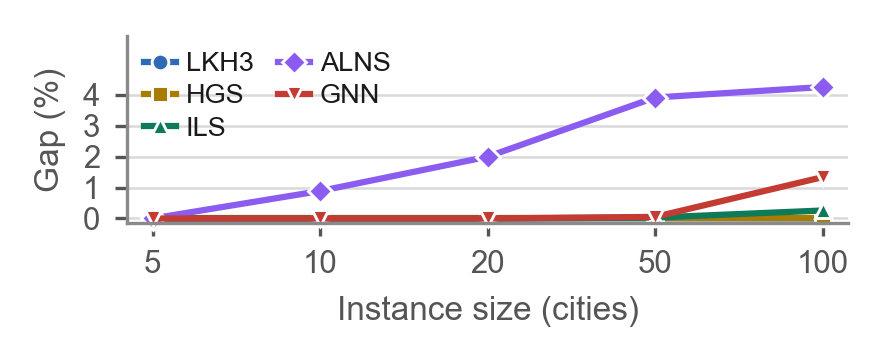
\includegraphics[width=0.92\columnwidth]{Figures/fig1_gap.png}
    \caption{Gap médio de otimalidade por tamanho de instância. Fonte: Produzido pelos autores.}
    \label{fig:gap}
\end{figure}

\begin{figure}[H]
    \centering
    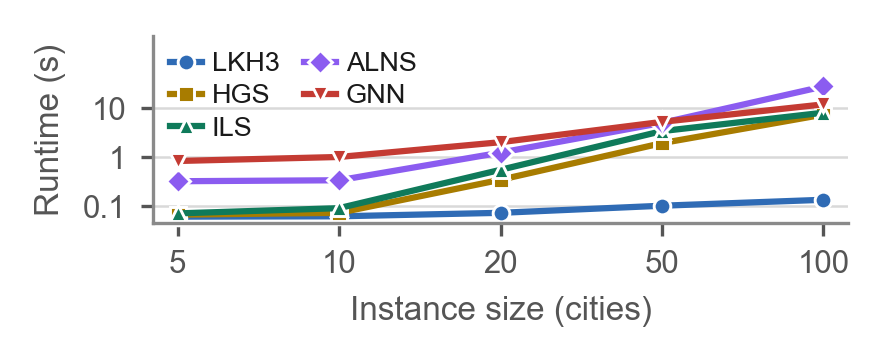
\includegraphics[width=0.92\columnwidth]{Figures/fig2_time.png}
    \caption{Tempo médio de execução em escala logarítmica. Fonte: Produzido
    pelos autores.}
    \label{fig:time}
\end{figure}

Considerando os dois eixos com dados de TSP100, a Figura~\ref{fig:tradeoff}
mostra que o LKH3 é o solver que melhor combina um bom gap médio de otimalidade de rota a um tempo
mais de 50 vezes menor que o do HGS, seu concorrente direto em qualidade.
A taxa de vitória apresentada na Figura~\ref{fig:winrate} evidencia que o empate
em qualidade entre os dois não é precisamente exato, já que o HGS devolveu a melhor rota em
100\% das execuções, contra 99\% do LKH3, mas a diferença permanece inferior
a 0,005\% do gap médio. Nota-se ainda que o ILS alcançou a melhor rota em 89\%
das execuções, a GNN em 79\% e o ALNS em apenas 49\%.

\begin{figure}[H]
    \centering
    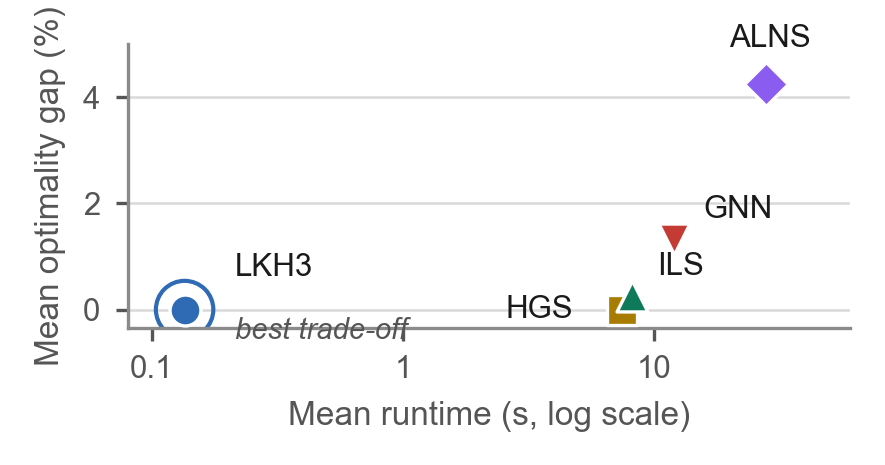
\includegraphics[width=0.92\columnwidth]{Figures/fig3_tradeoff.png}
    \caption{Qualidade versus tempo nas instâncias de 100 cidades; o LKH3 é o
    único solver não dominado. Fonte: Produzido pelos autores.}
    \label{fig:tradeoff}
\end{figure}

\begin{figure}[H]
    \centering
    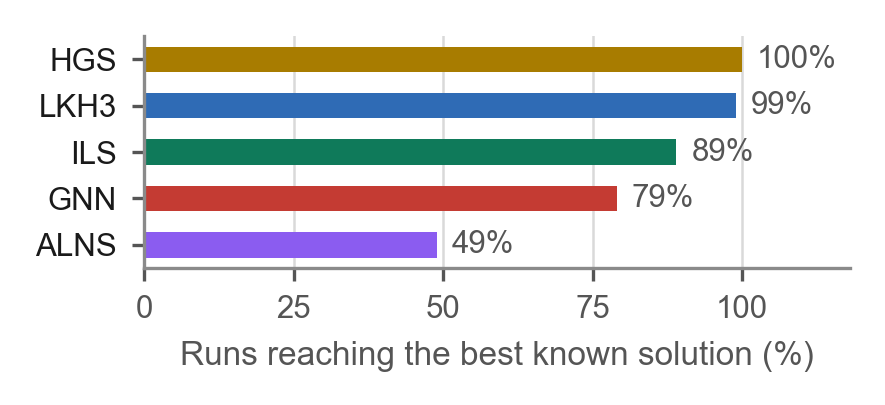
\includegraphics[width=0.92\columnwidth]{Figures/fig4_winrate.png}
    \caption{Porcentagem de execuções em que cada solver alcançou a melhor rota
    conhecida. Fonte: Produzido pelos autores.}
    \label{fig:winrate}
\end{figure}

\section{Conclusões}

Para o conjunto de instâncias avaliado, o LKH3 se mostra o melhor
solver no geral: é estatisticamente tão preciso quanto a melhor alternativa e
executa em uma fração de segundo, o melhor comportamento compatível com uma
aplicação. O HGS permanece como referência em qualidade de solução e
seria a alternativa natural sempre que o tempo de execução for irrelevante. O
ALNS foi o solver mais fraco nos dois eixos, e a GNN se mostra bastante
promissora, principalmente para instâncias maiores e assimétricas, mas ainda não
competitiva nessas escalas.

Os autores declaram não haver conflito de interesses.

Todos os autores aprovaram a versão final do resumo.

Esta pesquisa foi realizada com o apoio da Fundação de Amparo à Pesquisa do Estado de São Paulo (FAPESP).

\bibliography{bibtex/siicusp2026}

\end{document}
